\documentclass[twocolumn]{rbef}

\usepackage{lipsum}

\usepackage{bbm}
\usepackage{subfig}
\usepackage{pdfpages} % Para incluir a capa.

\hypersetup{%
    pdfborder = {0 0 0}
}

\newcommand{\1}{\mathbbm{1}}
\newcommand{\s}{\mathcal{S}}
\newcommand{\T}{\mathcal{T}}
\newcommand{\A}{\mathcal{A}}
\newcommand{\ket}{\rangle}
\newcommand{\bra}{\langle}

\newtheorem{defi}{Definição}
\newtheorem{theorem}{Teorema}
\newtheorem{acknowledgement}[theorem]{Acknowledgement}
\newtheorem{algorithm}[theorem]{Algorithm}
\newtheorem{axiom}[theorem]{Axiom}
\newtheorem{claim}[theorem]{Claim}
\newtheorem{conclusion}[theorem]{Conclusion}
\newtheorem{condition}[theorem]{Condition}
\newtheorem{conjecture}[theorem]{Conjecture}
\newtheorem{corollary}[theorem]{Corollary}
\newtheorem{criterion}[theorem]{Criterion}
\newtheorem{definition}[theorem]{Definition}
\newtheorem{example}[theorem]{Example}
\newtheorem{exercise}[theorem]{Exercise}
\newtheorem{lemma}[theorem]{Lemma}
\newtheorem{notation}[theorem]{Notation}
\newtheorem{problem}[theorem]{Problem}
\newtheorem{proposition}[theorem]{Proposition}
\newtheorem{remark}[theorem]{Remark}
\newtheorem{solution}[theorem]{Solution}
\newtheorem{summary}[theorem]{Summary}
\newenvironment{proof}[1][Proof]{\noindent\textbf{#1.} }{\ \rule{0.5em}{0.5em}}

\titulocabecalho{Utilizando a Regressão Logística para Classificação de Churn em Ambiente de Startup}
\autorcabecalho{Antonio C. da Silva Júnior}

\numeracao{01}
\volume{01}
\numero{01}
\ano{2019}
\doi{http://dsbd.leg.ufpr.br/tcc}
% \tipodeartigo{TCC DSBD}
\tipodeartigo{Especialização em Data Science \& Big Data}
% \addtocounter{page}{566} %% \setcounter produces extra white page!!! use ===\addtocounter===

\author[]{Antonio C. da Silva Júnior}

\affil[]{Campus Santos, Universidade Paulista Av. Conselheiro Nébias 766, Boqueirão, 11045-002, Santos, SP, Brasil\thanks{\href{emailto:juniorssz@gmail.com}{\href{mailto:juniorssz@gmail.com}{\nolinkurl{juniorssz@gmail.com}}}}
}
\titulo{Utilizando a Regressão Logística para Classificação de Churn em Ambiente de Startup}

\subtitulo{Using Logistic Regression for Customer Churn Classification in Startup Environment}

% -----------------------------------------------------------------------

\begin{document}

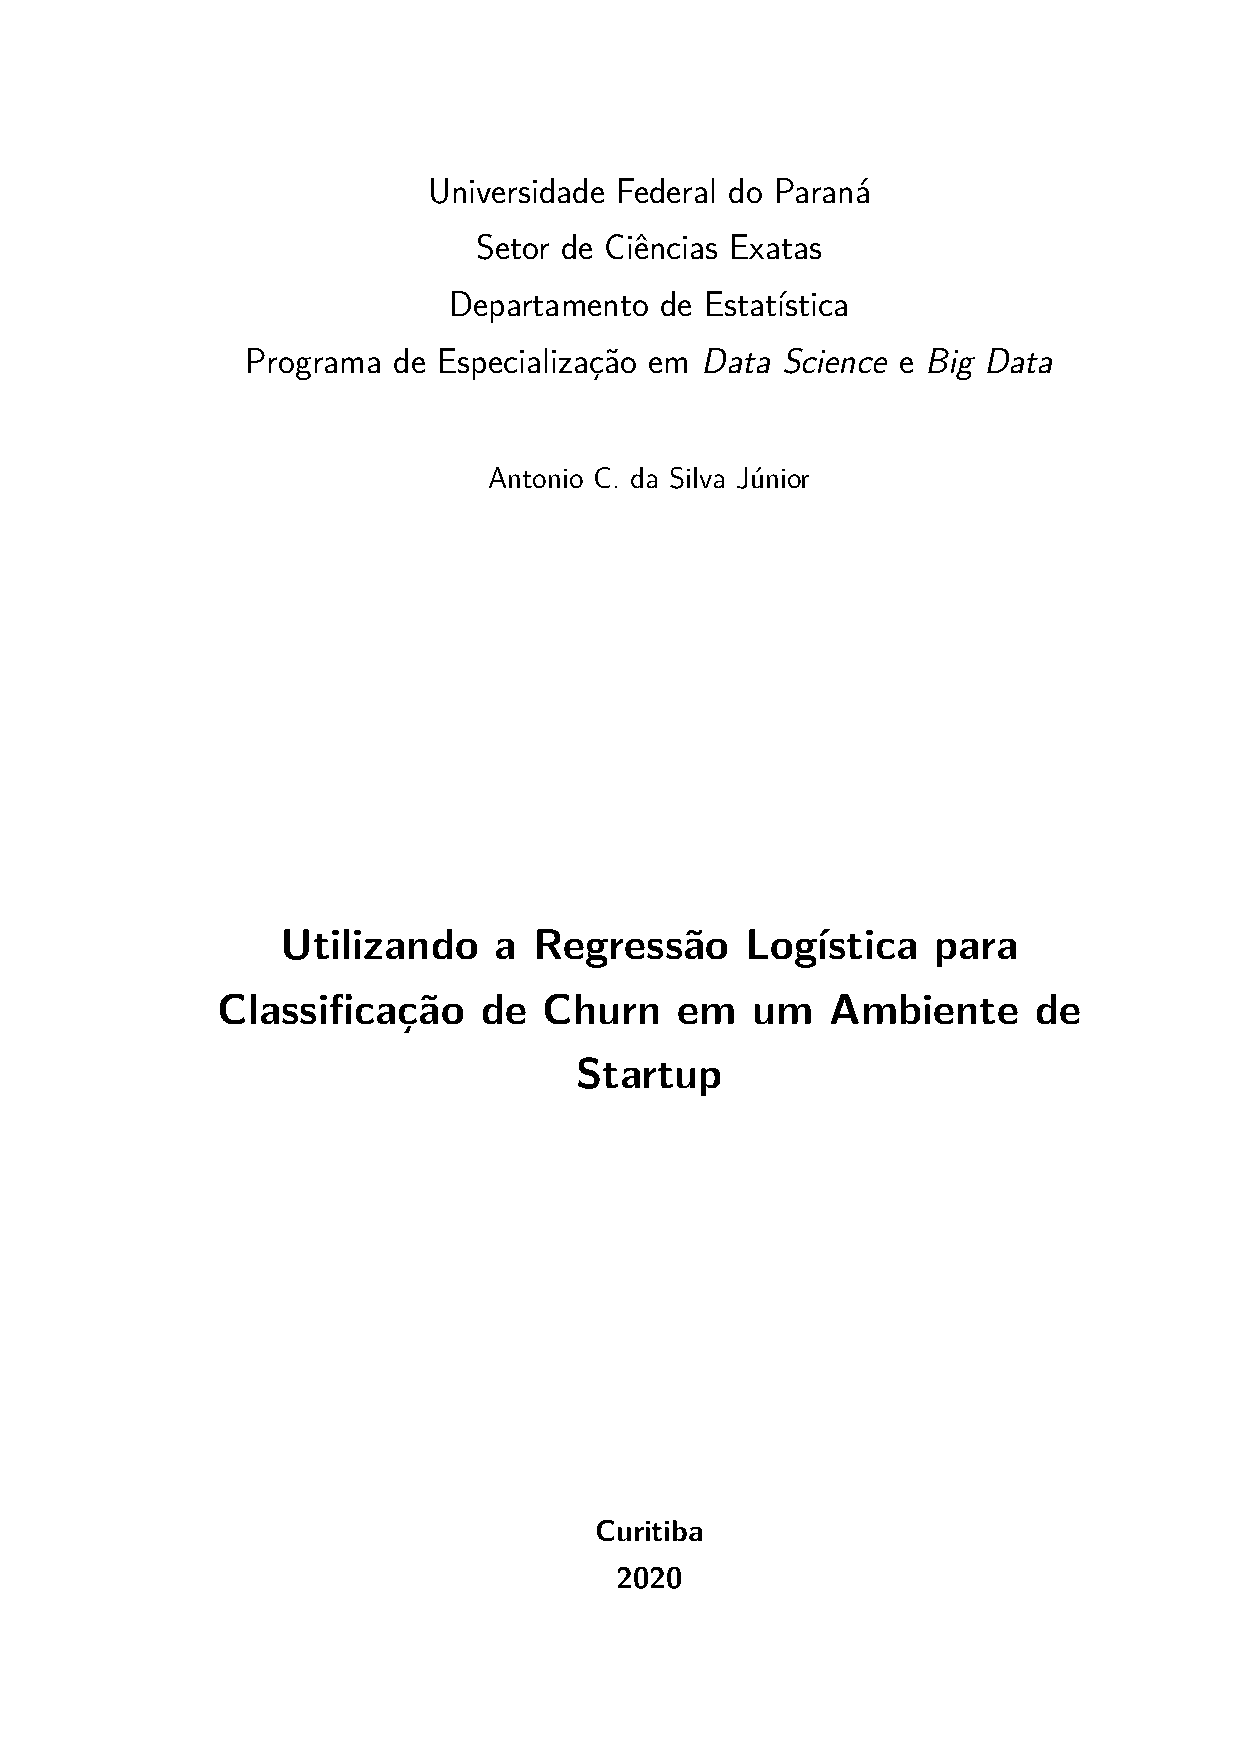
\includepdf[pages=-]{cover.pdf} % Incluí a capa

\begin{primeirapagina}

  % \begin{center}
  %   \vspace{-12pt} \small{Recebido em xxx. Aceito em xxx}
  % \end{center}

  \begin{abstract}
    asdfasdf.
    \palavraschave{asdfasdf, asdfasdf, asdfasdf, asdfasdf, asdfasdf}

  \end{abstract}

  \begin{otherlanguage}{english}

    \begin{abstract}
      asdfasdf.
      \keywords{asdfasdf, asdfasdf, asdfasdf, asdfasdf, asdfasdf}

    \end{abstract}
  \end{otherlanguage}

\end{primeirapagina}
\saythanks

\hypertarget{introduuxe7uxe3o}{%
\section{Introdução}\label{introduuxe7uxe3o}}

A importância do relacionamento de longo prazo entre cliente e empresa é um assunto vastamente discutido na literatura. Devido aos efeitos do aprendizado e à redução dos custos de manutenção, atender um cliente se torna menos dispendioso a cada ano adicional de relacionamento \cite{Ganesh2000}. Por conta do aumento dos custos para atração de novos clientes em um mercado competitivo e à potencial redução dos custos associados aos relacionamentos de longo prazo, a retenção de clientes se torna essencial para a sobrevivência e o sucesso econômico das empresas do setor de serviços \cite{HennigThurau2004}. De acordo com \cite{Gallo2014}, dependendo do estudo e do segmento no qual a empresa está inserida, o custo para adquirir um novo cliente pode ser de cinco a vinte e cinco vezes superior ao da manutenção de um cliente já existente.

O desenvolvimento de estratégias para retenção de clientes se tornou uma prática comum entre empresas de diversos segmentos, e em consequência, antever o abandono de clientes se tornou um anseio constante. Em um momento de generalizada de esforços na direção da cultura orientada a dados, os modelos preditivos para detecção de abandono de clientes, predominantemente utilizados por grandes companhias no setor de telecomunicações, se tornaram ferramentas populares nas empresas, independentemente da magnitude e da área de atuação.

A literatura comprova que a modelagem preditiva de abandono de clientes, também conhecida como modelagem preditiva de churn, é um tema bastante explorado e que possibilita inúmeras maneiras de desfecho: Botelho e Tostes \cite{Botelho2010} ajustaram um modelo de regressão logística para predizer a probabilidade de churn em uma grande empresa de varejo; Vafeiadis et al.~\cite{Vafeiadis2015} tiveram sucesso, entre os métodos comparados, na classificação de churn através do SVM (kernel polinomial) com AdaBoost em uma empresa de telecomunicações; Baseados nos dados de avaliações online de clientes, Kumar e Yadav \cite{Kumar2020} propuseram um modelo preditivo de churn baseado em regras através de redes neurais artificiais e teoria dos conjuntos aproximados.

Com base nos dados de uma startup brasileira que tem como principal produto uma plataforma digital para conectar vendedores de diversos segmentos aos grandes marketplaces, a proposta deste artigo é apresentar um modelo preditivo que possibilite não só a classificação de vendedores propensos a abandonar a empresa, mas que também permita a interpretação dos motivos que possivelmente estejam impactando a predição. Diante da variedade de técnicas disponíveis e das particularidades de cada modelo de negócio, a escolha do algoritmo adequado se torna uma etapa crucial do processo de modelagem. Portanto, tendo como referência a abordagem de \cite{Junior2020}, que utilizaram uma modelagem híbrida multicritério considerando múltiplos decisores para a escolha de um modelo preditivo de churn, o algoritmo escolhido para desenvolver o classificador proposto foi a regressão logística.

\hypertarget{materiais-e-muxe9todos}{%
\section{Materiais e métodos}\label{materiais-e-muxe9todos}}

\hypertarget{estruturauxe7uxe3o-do-conjunto-de-dados}{%
\subsection{Estruturação do conjunto de dados}\label{estruturauxe7uxe3o-do-conjunto-de-dados}}

Os dados utilizados neste trabalho referem-se a clientes de uma startup paranaense, anonimizados e com variáveis quantitativas padronizadas com média 0 e desvio padrão 1. Considerando que estes clientes contrataram uma plataforma digital que possibilita a venda de produtos nos principais marketplaces, neste trabalho eles serão chamados de vendedores. Devido às características da arquitetura do banco de dados e às particularidades do negócio da companhia, houve a necessidade de realizar um longo processo de data wrangling. Este processo inicia-se por um diagnóstico preliminar dos dados, ou seja, se estão no formato adequado, se respondem as perguntas que motivaram a análise e o que é necessário para colocá-los no formato ideal. Em seguida avalia-se a ocorrência de dados faltantes, valores inconsistentes e duplicatas e, por fim, realiza-se um processo de limpeza e transformação, de modo a se obter um conjunto de dados adequado para o estudo \cite{Kandel2011}.

\hypertarget{definiuxe7uxe3o-da-resposta-e-covariuxe1veis-de-desempenho}{%
\subsubsection{Definição da resposta e covariáveis de desempenho}\label{definiuxe7uxe3o-da-resposta-e-covariuxe1veis-de-desempenho}}

Inicialmente foram definidos como churn (\(Y=1\)) os vendedores que estiveram inativos por 30 dias corridos desde a data da última atividade e permaneceram no mesmo estado em definitivo, considerando como atividade o acesso à plataforma digital ou a ocorrência de uma venda online. Em seguida, em função da data de corte estabelecida conforme a Tabela \ref{tab:dataDeCorte}, foram mantidos no conjunto de dados somente os vendedores com pelo menos 90 dias de histórico. O período de 90 dias, finalizado na data de corte, foi dividido igualmente em dois subperíodos, onde foram calculadas métricas como faturamento, ticket médio, quantidade de produtos publicados, quantidade de pedidos cancelados, número de dias em atividade e etc., em cada cada um dos subperíodos. Em seguida, através da Equação \eqref{eq:desempenho}, foi calculado desempenho do vendedor em função de diversas métricas, onde \(V1\) e \(V2\) são os valores calculados para cada subperíodo.

As métricas desempenho, data à natureza da equação de origem, possuem o comportamento explicado pela Tabela \ref{tab:metricas}. Ao término desta etapa foi obtido um conjunto de dados composto pela variável resposta (churn) e, como covariáveis, 10 métricas de desempenho, onde cada observação representa um vendedor.

\begin{table}

\caption{\label{tab:dataDeCorte}Definição da data de corte}
\centering
\fontsize{10}{12}\selectfont
\begin{tabular}[t]{ll}
\toprule
Vendedor & Data de corte\\
\midrule
Definido como churn & Última atividade\\
Em atividade normal & Realização da análise\\
\bottomrule
\end{tabular}
\end{table}

\begin{equation}
Desempenho = \dfrac{V2}{V1+V2} \label{eq:desempenho}
\end{equation}

\begin{table}

\caption{\label{tab:metricas}Interpretação das métricas de desempenho}
\centering
\fontsize{10}{12}\selectfont
\begin{tabular}[t]{ll}
\toprule
Valor & Desempenho\\
\midrule
0,5 & Mantido\\
> 0,5 & Aumentado\\
< 0,5 & Reduzido\\
\bottomrule
\end{tabular}
\end{table}

\hypertarget{adiuxe7uxe3o-de-outras-covariuxe1veis}{%
\subsubsection{Adição de outras covariáveis}\label{adiuxe7uxe3o-de-outras-covariuxe1veis}}

Foram adicionadas covariáveis qualitativas que representam o estágio do vendedor, o plano contratado e a região de origem, bem como covariáveis quantitativas como o faturamento total, total de produtos publicados, quantidade total de pedidos e etc., resultando em um conjunto de dados com 26 covariáveis.

\hypertarget{criauxe7uxe3o-de-covariuxe1veis-binuxe1rias}{%
\subsubsection{Criação de covariáveis binárias}\label{criauxe7uxe3o-de-covariuxe1veis-binuxe1rias}}

Dada a necessidade de analisar o comportamento da variável resposta em função de uma covariável qualitativa com \(n\) categorias, deve-se criar \(n-1\) covariáveis binárias (dummies), que assumem valores iguais a 0 ou 1, ficando por conta do pesquisador decidir qual das categorias será a referência (dummy = 0) \cite{Favero2017}. Portanto, as covariáveis qualitativas adicionadas foram transformadas em binárias, resultando em um conjunto de dados composto por 35 variáveis e 11.131 observações.

\hypertarget{modelos-de-regressuxe3o-loguxedstica-binuxe1ria}{%
\subsection{Modelos de regressão logística binária}\label{modelos-de-regressuxe3o-loguxedstica-binuxe1ria}}

O objetivo da regressão logística binária é o estudo da probabilidade de ocorrência de um evento de interesse (\(Y\)), apresentado na forma dicotômica (\(Y=1\) se o evento de interesse ocorrer; \(Y=0\), caso contrário), em função de um vetor vetor de covariáveis (\(X_1, ..., X_n\)). Sua definição ocorre através da Equação \eqref{eq:logito}, onde \(\beta_j\) (\(j = 0,1,2,...,p\)) representam os parâmetros a serem estimados, sendo \(\beta_0\) o intercepto e os demais, parâmetros de cada covariável, e o subscrito \(i\) representa cada observação da amostra (\(i = 1, 2,...,n\)) \cite{Favero2017}.
\begin{equation}
ln \left ( \dfrac{\pi_i}{1-\pi_i} \right ) = \beta_0 + \beta_1 X_{i1} + ... +  \beta_p X_{ip}\label{eq:logito}
\end{equation}

A Equação \eqref{eq:logito}, conhecida como logito, modela a log-chance de ocorrência do evento de interesse. Portanto, para obter uma expressão para a probabilidade de ocorrência do evento é necessário isolar matematicamente \(\pi_i\), resultando na Equação \eqref{eq:probabilidade}.
\begin{equation}
\pi_i = \dfrac{1}{1 + e^{-(\beta_0 + \beta_1 X_{i1} + ... +  \beta_p X_{ip})}}\label{eq:probabilidade}
\end{equation}

A estimação dos parâmetros \(\beta_i\) é realizada por máxima verossimilhança, método que consiste em encontrar, através da programação linear, os parâmetros que maximizam a função de verossimilhança representada através da Equação \eqref{eq:verossimilhanca}.
\begin{equation}
L =  \prod_{i=1}^{n} \left[ \pi^{Y_i} (1-\pi_i)^{1-Y_i} \right]\label{eq:verossimilhanca}
\end{equation}

Entretanto, matematicamente é mais conveniente trabalhar com o logaritmo da função de verossimilhança, conhecido como função de log-verossimilhança \cite{Favero2017,Botelho2010}, representado através da Equação \eqref{eq:logverossimilhanca}.

\begin{equation}
logL = \sum_{i=1}^{n} \left\{ \big[Y_iln(\pi_i)\big] + \big[(1-Y_i)ln(1-\pi_i)\big] \right\}\label{eq:logverossimilhanca}
\end{equation}

\hypertarget{seleuxe7uxe3o-de-covariuxe1veis-atravuxe9s-do-algoritmo-stepwise}{%
\subsection{Seleção de covariáveis através do algoritmo stepwise}\label{seleuxe7uxe3o-de-covariuxe1veis-atravuxe9s-do-algoritmo-stepwise}}

A comparação entre dois modelos pode ser realizada através do Critério de Informação de Akaike (AIC), definido por \(-2logL + 2p\), onde \(logL\) é a log-verossimilhança maximizada e \(p\) é o número de parâmetros do modelo, devendo-se selecionar o modelo que apresentar o menor valor de AIC. Entretanto, avaliar todas a regressões possíveis, mesmo para um número moderado de covariáveis, pode ser computacionalmente invivável, mas como alternativa é possível utilizar o algoritmo \textit{stepwise}, que funciona da seguinte forma \cite{Taconeli2019}:

\begin{enumerate}
\def\labelenumi{\arabic{enumi}.}
\item
  Ajuste do modelo com todas as covariáveis;
\item
  Avaliação tanto a exclusão como a inclusão de cada covariável, através do cálculo do AIC;
\item
  Exclusão (ou inclusão) da covariável cuja exclusão (ou inclusão) resulta em menor AIC;
\item
  Repete-se os passos 1 a 3 para o novo modelo e o processo continua até que nenhuma exclusão (ou inclusão) que resulte em menor AIC.
\end{enumerate}

\hypertarget{validauxe7uxe3o-cruzada-por-k-fold}{%
\subsection{Validação cruzada por K-fold}\label{validauxe7uxe3o-cruzada-por-k-fold}}

A validação cruzada por k-fold é uma técnica de reamostragem aplicada com o propósito de reduzir o vício e a variância do modelo, que funciona da seguinte forma \cite{Kohavi1995}:

\begin{enumerate}
\def\labelenumi{\arabic{enumi}.}
\item
  Separação aleatória dos dados de treino em \(k\) partições de tamanho aproximadamente igual (folds);
\item
  Isolamento de uma das partições e treino do modelo com os dados das demais partições concatenadas;
\item
  Validação do modelo com os dados da partição isolada, através de determinada métrica de avaliação;
\item
  Repete-se os passos 2 e 3 até que o modelo seja validado em todas as \(k\) partições;
\item
  A métricas de avaliação de cada iteração são resumidas, normalmente através da média aritmética.
\end{enumerate}

\hypertarget{ajuste-do-modelo-de-regressuxe3o-loguxedstica-binuxe1ria}{%
\subsection{Ajuste do modelo de regressão logística binária}\label{ajuste-do-modelo-de-regressuxe3o-loguxedstica-binuxe1ria}}

\begin{table*}

\caption{\label{tab:covars}Covariáveis utilizadas pelo modelo}
\centering
\fontsize{10}{12}\selectfont
\begin{tabular}[t]{lll}
\toprule
Variável & Descrição & Medição\\
\midrule
\addlinespace[0.3em]
\multicolumn{3}{l}{\textbf{Métricas de desempenho}}\\
\hspace{1em}x1 & Desempenho do número de pedidos no período & percentual\\
\hspace{1em}x2 & Desempenho do número de dias em atividade no período & percentual\\
\hspace{1em}x3 & Desempenho do número de pedidos cancelados ou suspensos no período & percentual\\
\hspace{1em}x5 & Desempenho da média de dias de atraso (postagens) no período & percentual\\
\hspace{1em}x6 & Desempenho da média de dias de atraso (entregas) no período & percentual\\
\hspace{1em}x7 & Desempenho do faturamento no período & percentual\\
\hspace{1em}x10 & Desempenho do ticket médio no período & percentual\\
\addlinespace[0.3em]
\multicolumn{3}{l}{\textbf{Qualitativas}}\\
\hspace{1em}x12 & Necessita de dias adicionais para postagem & 1 = sim; 0 = não\\
\hspace{1em}x13 & Está no estágio B & 1 = sim; 0 = não\\
\hspace{1em}x14 & Esta no estágio I & 1 = sim; 0 = não\\
\hspace{1em}x15 & Está no estágio R & 1 = sim; 0 = não\\
\hspace{1em}x17 & Possui o plano M & 1 = sim; 0 = não\\
\hspace{1em}x21 & Localizado na região Sudeste & 1 = sim; 0 = não\\
\addlinespace[0.3em]
\multicolumn{3}{l}{\textbf{Quantitativas}}\\
\hspace{1em}x23 & Valor do fluxo de caixa & contínua\\
\hspace{1em}x25 & Valor total do faturamento & contínua\\
\hspace{1em}x30 & Número total de produtos publicados & discreta\\
\hspace{1em}x32 & Número de dias desde a contratação até a primeira venda & discreta\\
\hspace{1em}x33 & Número de dias desde a contratação até estar pronto para operar & discreta\\
\hspace{1em}x34 & Número de dias em atividade no período & discreta\\
\bottomrule
\end{tabular}
\end{table*}

O conjunto de dados foi separado aleatoriamente em duas partes, garantindo a proporção aproximada de 47,3\% de ocorrência de churn (\(Y=1\)) em ambas as amostras. A amostra maior, com 75\% dos dados, foi utilizada para o ajuste de dois modelos à partir de todas as covariáveis disponíveis. Um deles, denominado \textit{modelo completo}, foi ajustado da maneira tradicional, ao passo que o segundo modelo, denominado \textit{modelo restrito}, teve o ajuste realizado através do algoritmo \textit{stepwise}.

Através do teste da razão da verossimilhança, representado através da Equação \eqref{eq:trv}, é possível verificar a qualidade do ajuste do \textit{modelo completo}, ajustado com \(j\) covariáveis, em comparação com o \textit{modelo restrito}, ajustado com \(j-k\) covariáveis, sendo \(k\) o número de covariáveis removidas do ajuste \cite{Favero2017}.

\begin{equation}
TRV = -2(logL_{completo} - logL_{restrito})\label{eq:trv}
\end{equation}

Quando a estatística do \(TRV\) é inferior ao valor da distribuição do \({\chi}^2\) com \(k\) graus de liberdade e 5\% de significância, não rejeitamos a hipótese nula, ou seja, concluimos que a remoção de \(k\) covariáveis não afeta a qualidade do ajuste do modelo. Ao realizar o teste, foi constatado que a remoção das 14 covariáveis, no \textit{modelo restrito}, não alterou a qualidade do ajuste, uma vez que a estatística do teste foi inferior ao valor da distribuição do \({\chi}^2\) com 14 graus de liberdade e 5\% de significância. Portanto, optou-se pelo \textit{modelo restrito} para a continuidade do estudo, uma vez que este possui complexidade inferior com relação ao \textit{modelo completo}, sem perda de qualidade. A Tabela \ref{tab:covars} exibe as 19 covariáveis selecionadas para o modelo.

\begin{figure}

{\centering 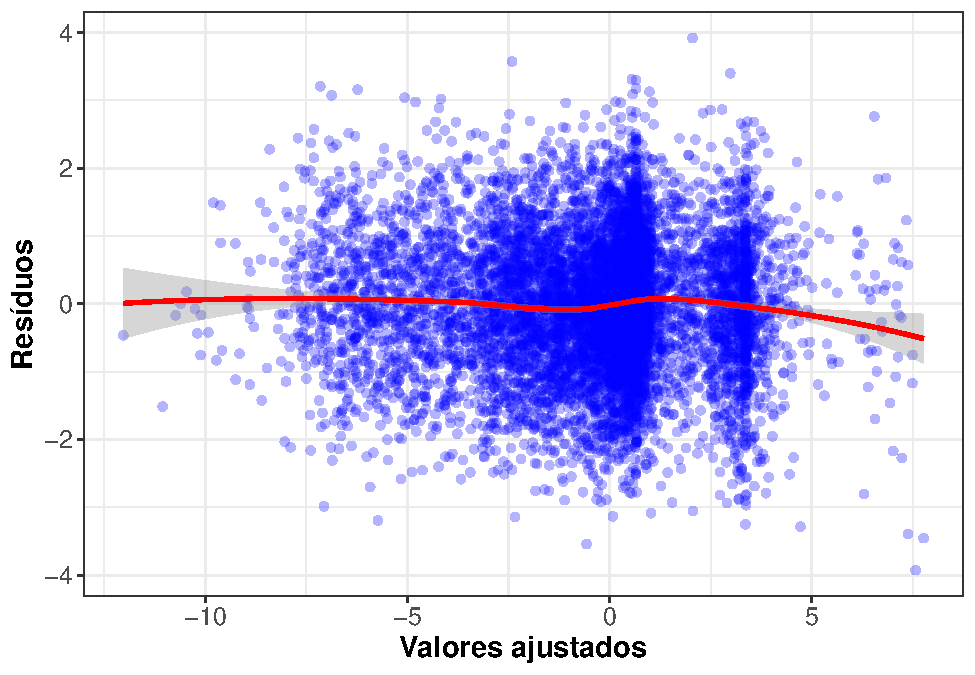
\includegraphics[width=1\linewidth]{article_files/figure-latex/resplot-1} 

}

\caption{Gráficos dos resíduos versus valores ajustados}\label{fig:resplot}
\end{figure}

\begin{figure}

{\centering 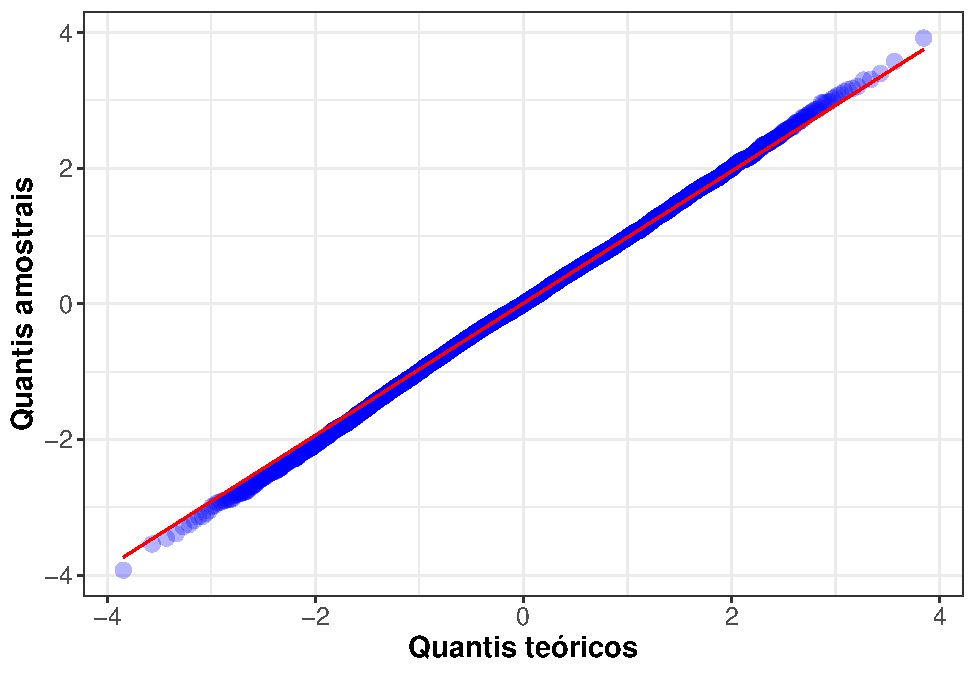
\includegraphics[width=1\linewidth]{article_files/figure-latex/qqplot-1} 

}

\caption{Gráfico quantil-quantil}\label{fig:qqplot}
\end{figure}

Com a intenção de generalizar o método de análise dos resíduos da regressão linear para todos os modelos lineares generalizados, Dunn e Smyth \cite{Dunn1996} propuseram os resíduos quantílicos aleatorizados, definidos por \(r_i = \phi^{-1}(u_i)\), onde \(\phi^{-1}\) é a inversa da função de distribuição acumulada da normal padrão e \(u_i = F(y_i;\mu_i,\phi)\), com distribuição uniforme entre 0 e 1, é calculado com base na distribuição acumulada do modelo proposto. Caso o modelo logístico esteja bem ajustado, espera-se resíduos quantílicos aleatorizados se apresentem normalmente distribuídos e com variância constante \cite{Taconeli2015}.

A análise da qualidade do ajuste, através dos resíduos, foi realizada de forma gráfica. Ao comparar os resíduos com os valores ajustados (Figura \ref{fig:resplot}) é possível observar que estes apresentam variabilidade aproximadamente constante e estão centrados predominantemente em 0, entre -2 e 2. No gráfico quantil-quantil \cite{Wilk1968} (Figura \ref{fig:qqplot}) nota-se que os resíduos estão, de forma razoável, aderentes à distribuição normal. Portanto, pode-se considerar que o modelo está bem ajustado.

\hypertarget{anuxe1lise-e-interpretauxe7uxe3o-dos-coeficientes}{%
\subsubsection{Análise e interpretação dos coeficientes}\label{anuxe1lise-e-interpretauxe7uxe3o-dos-coeficientes}}

asdfasdf

\hypertarget{avaliauxe7uxe3o-do-poder-preditivo-do-modelo}{%
\subsubsection{Avaliação do poder preditivo do modelo}\label{avaliauxe7uxe3o-do-poder-preditivo-do-modelo}}

asdfasdf

\hypertarget{conclusuxf5es}{%
\section{Conclusões}\label{conclusuxf5es}}

asdfasdf

\bibliographystyle{unsrt}
\bibliography{referencias}

\end{document}
